\chapter{Panels illumination}\label{appendix1}
The illumination of cosmic hits on all twelve panels in the first station, as described in Section \ref{eventselection}. 
The patterns are similar across all panels, with differences arising from the varying rotations of the panels relative to the station's center.
\begin{figure}[!h]
    \centering
    \begin{subfigure}[b]{0.4\textwidth}
        \centering
        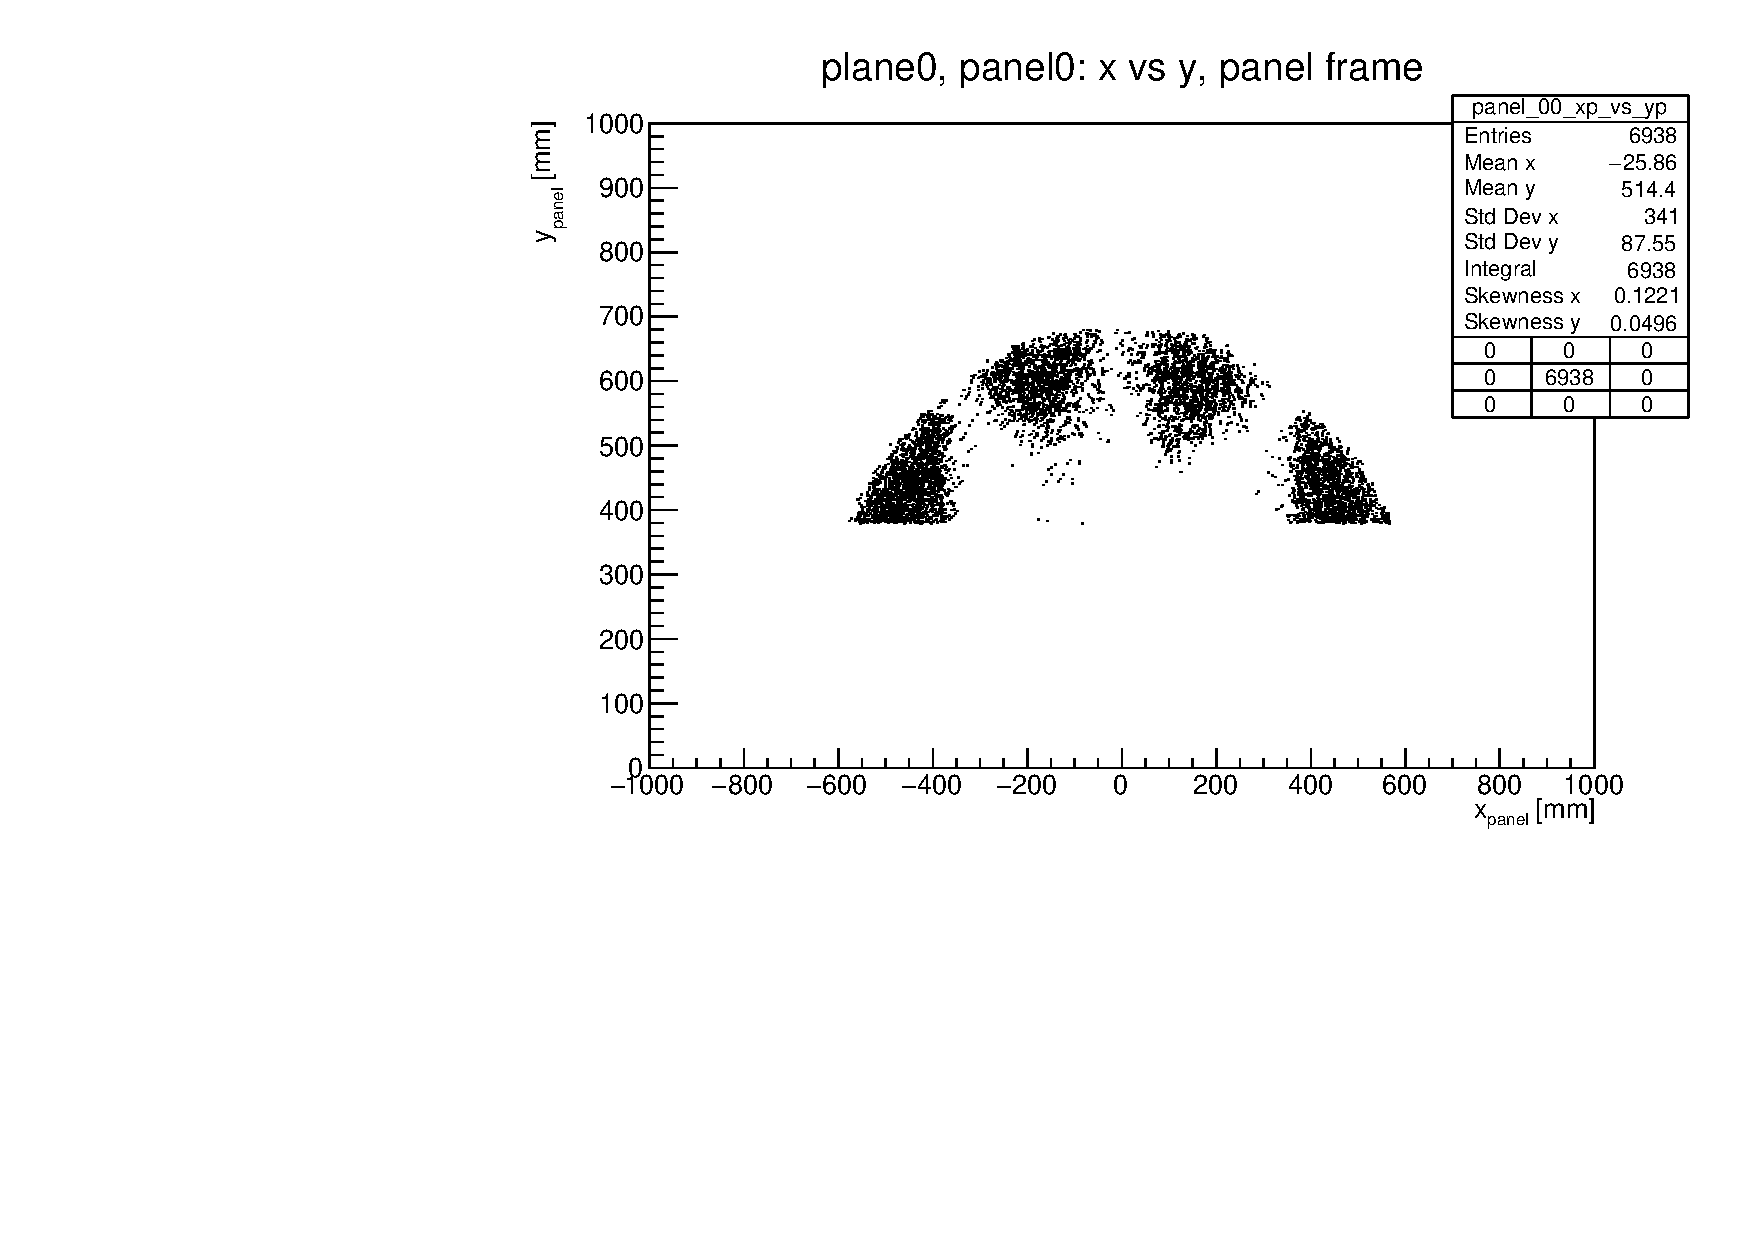
\includegraphics[width=0.95\textwidth]{figures/pdf/plane0_panel0_x_vs_y_all.pdf}
        %\caption{panel0}
        \label{fig:panel0plane0}
    \end{subfigure}
    \hfill
    \begin{subfigure}[b]{0.4\textwidth}
        \centering
        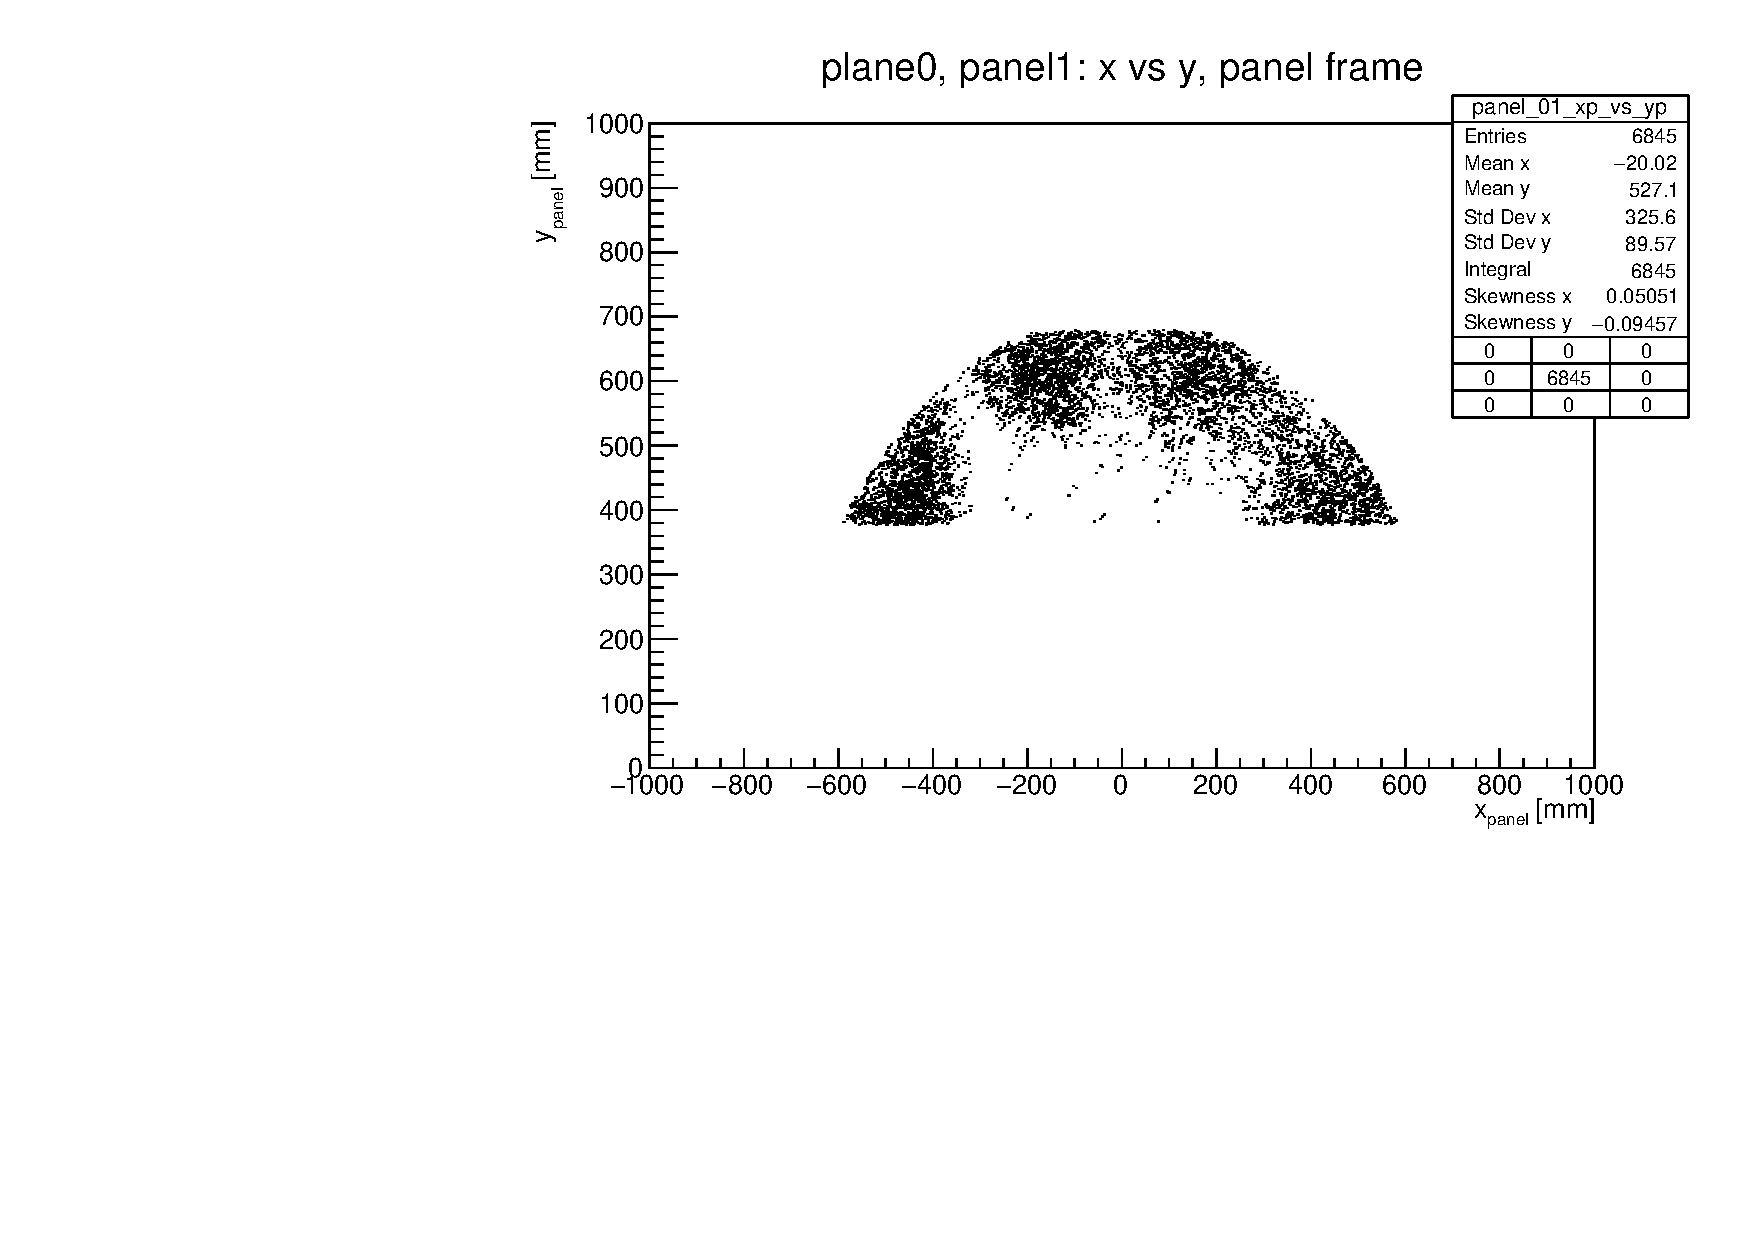
\includegraphics[width=0.95\textwidth]{figures/pdf/plane0_panel1_x_vs_y_all.pdf}
        %\caption{panel1}
        \label{fig:panel1plane0}
    \end{subfigure}
    \hfill
    \begin{subfigure}[b]{0.4\textwidth}
        \centering
        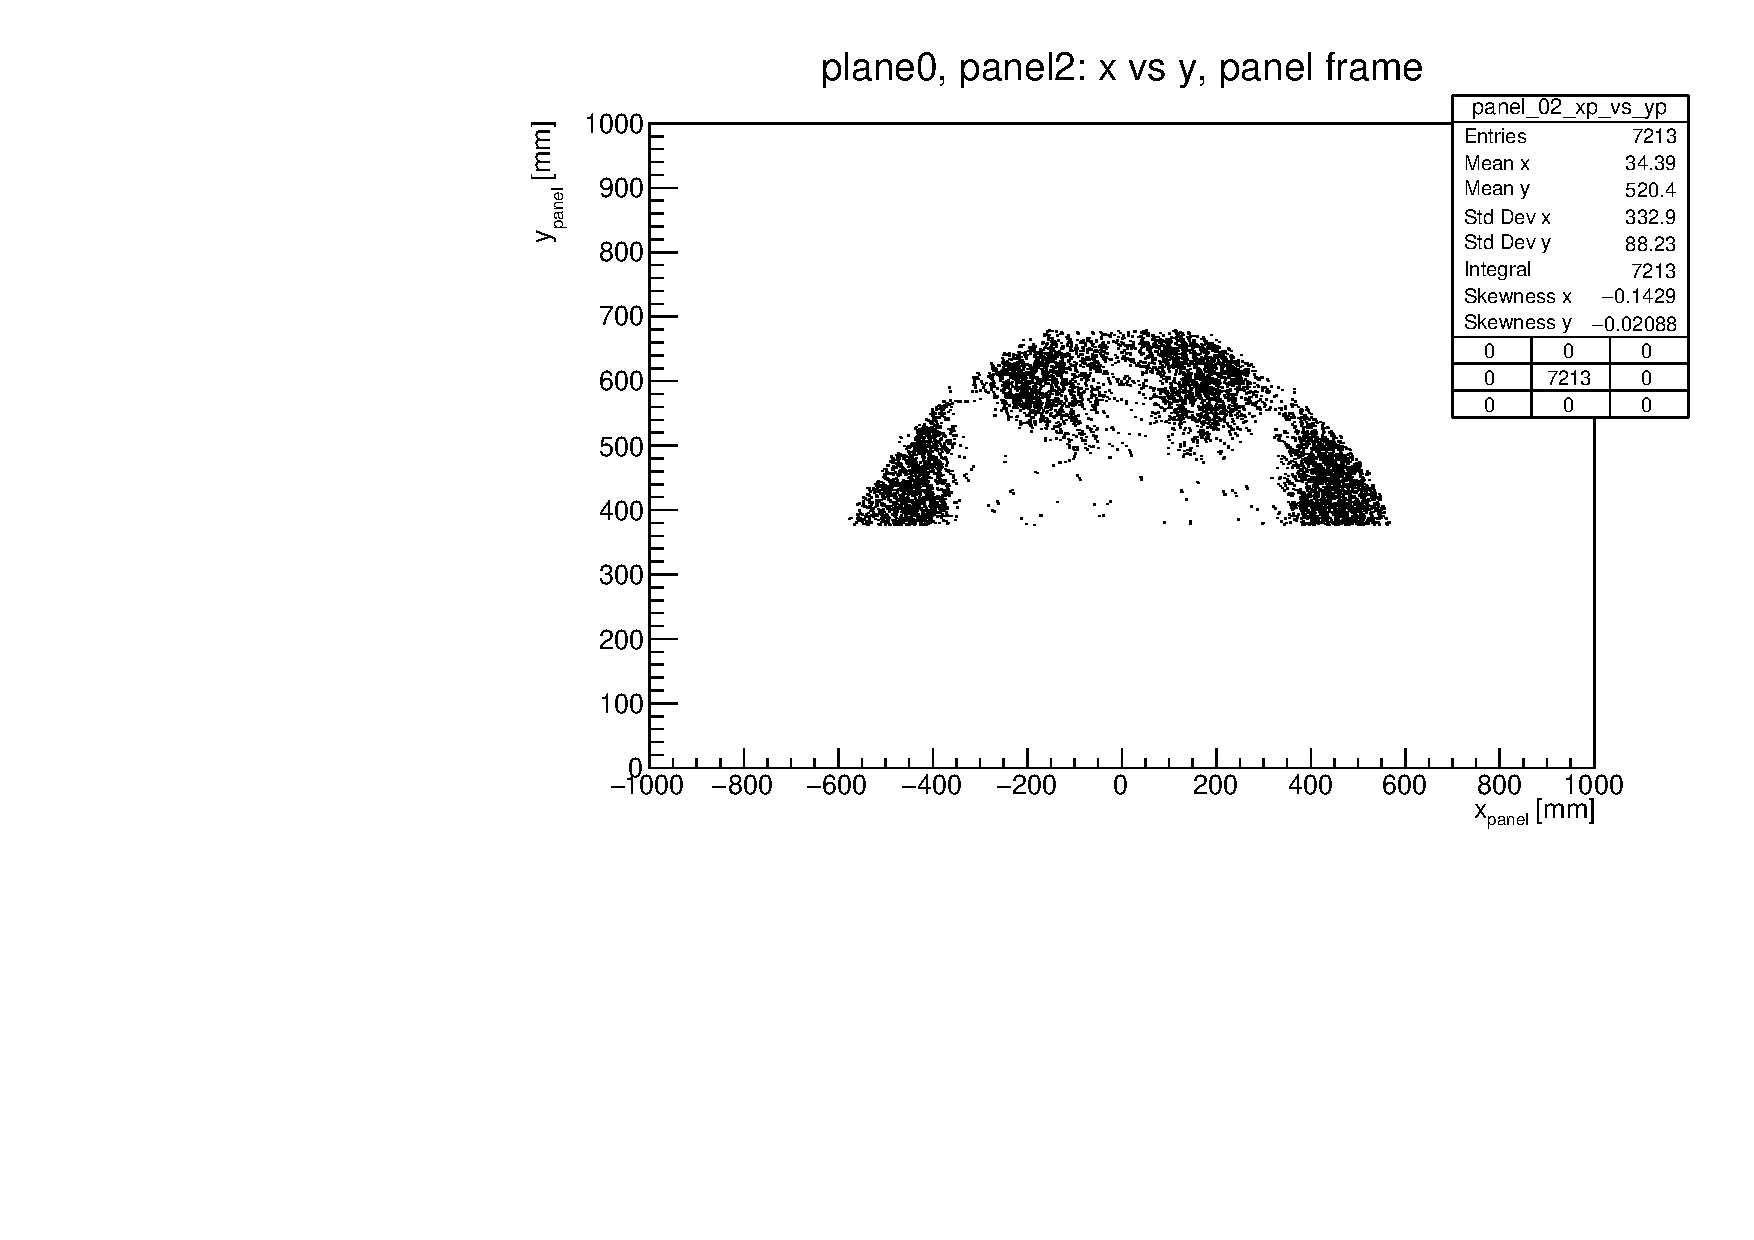
\includegraphics[width=0.95\textwidth]{figures/pdf/plane0_panel2_x_vs_y_all.pdf}
        %\caption{panel2}
        \label{fig:panel2plane0}
    \end{subfigure}
    \hfill
    \begin{subfigure}[b]{0.4\textwidth}
        \centering
        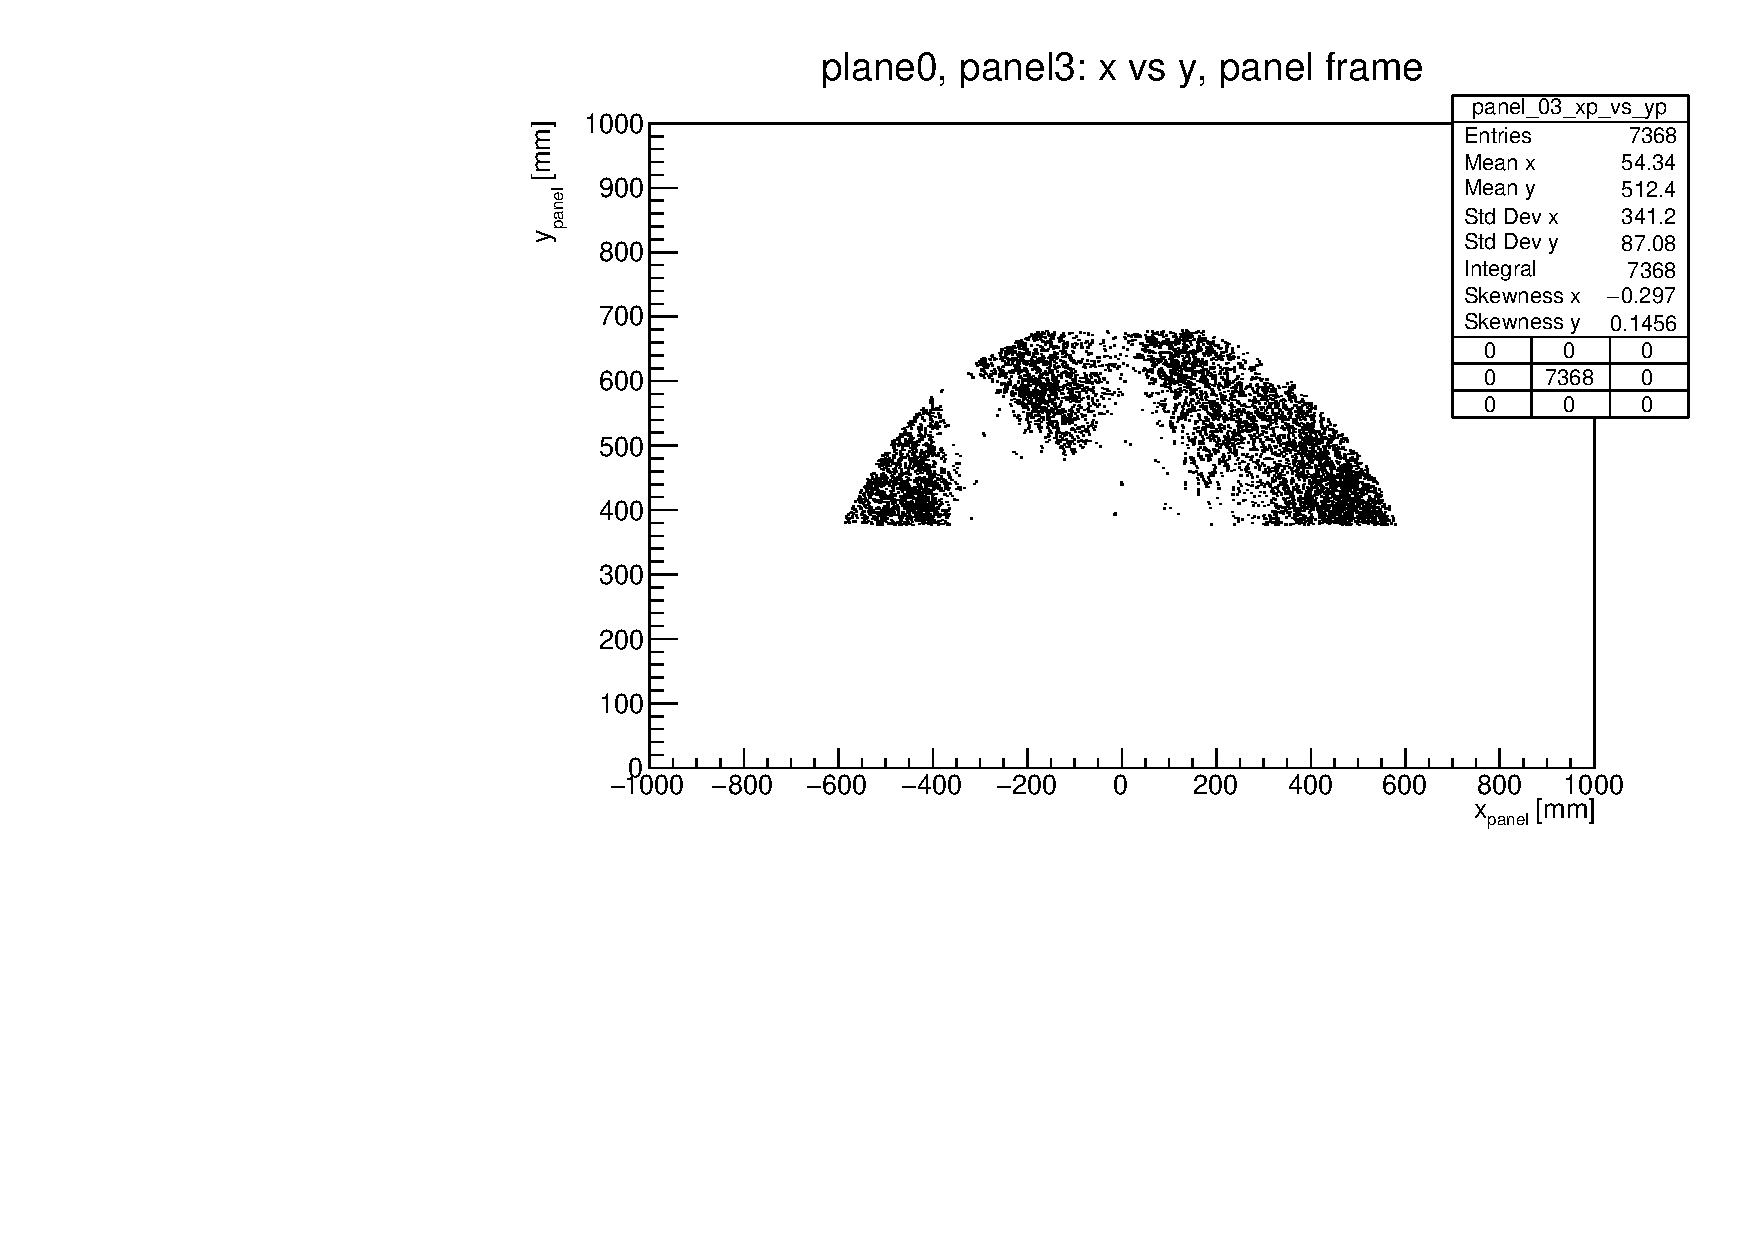
\includegraphics[width=0.95\textwidth]{figures/pdf/plane0_panel3_x_vs_y_all.pdf}
        %\caption{panel3}
        \label{fig:panel3plane0}
    \end{subfigure}
    \hfill
    \begin{subfigure}[b]{0.4\textwidth}
        \centering
        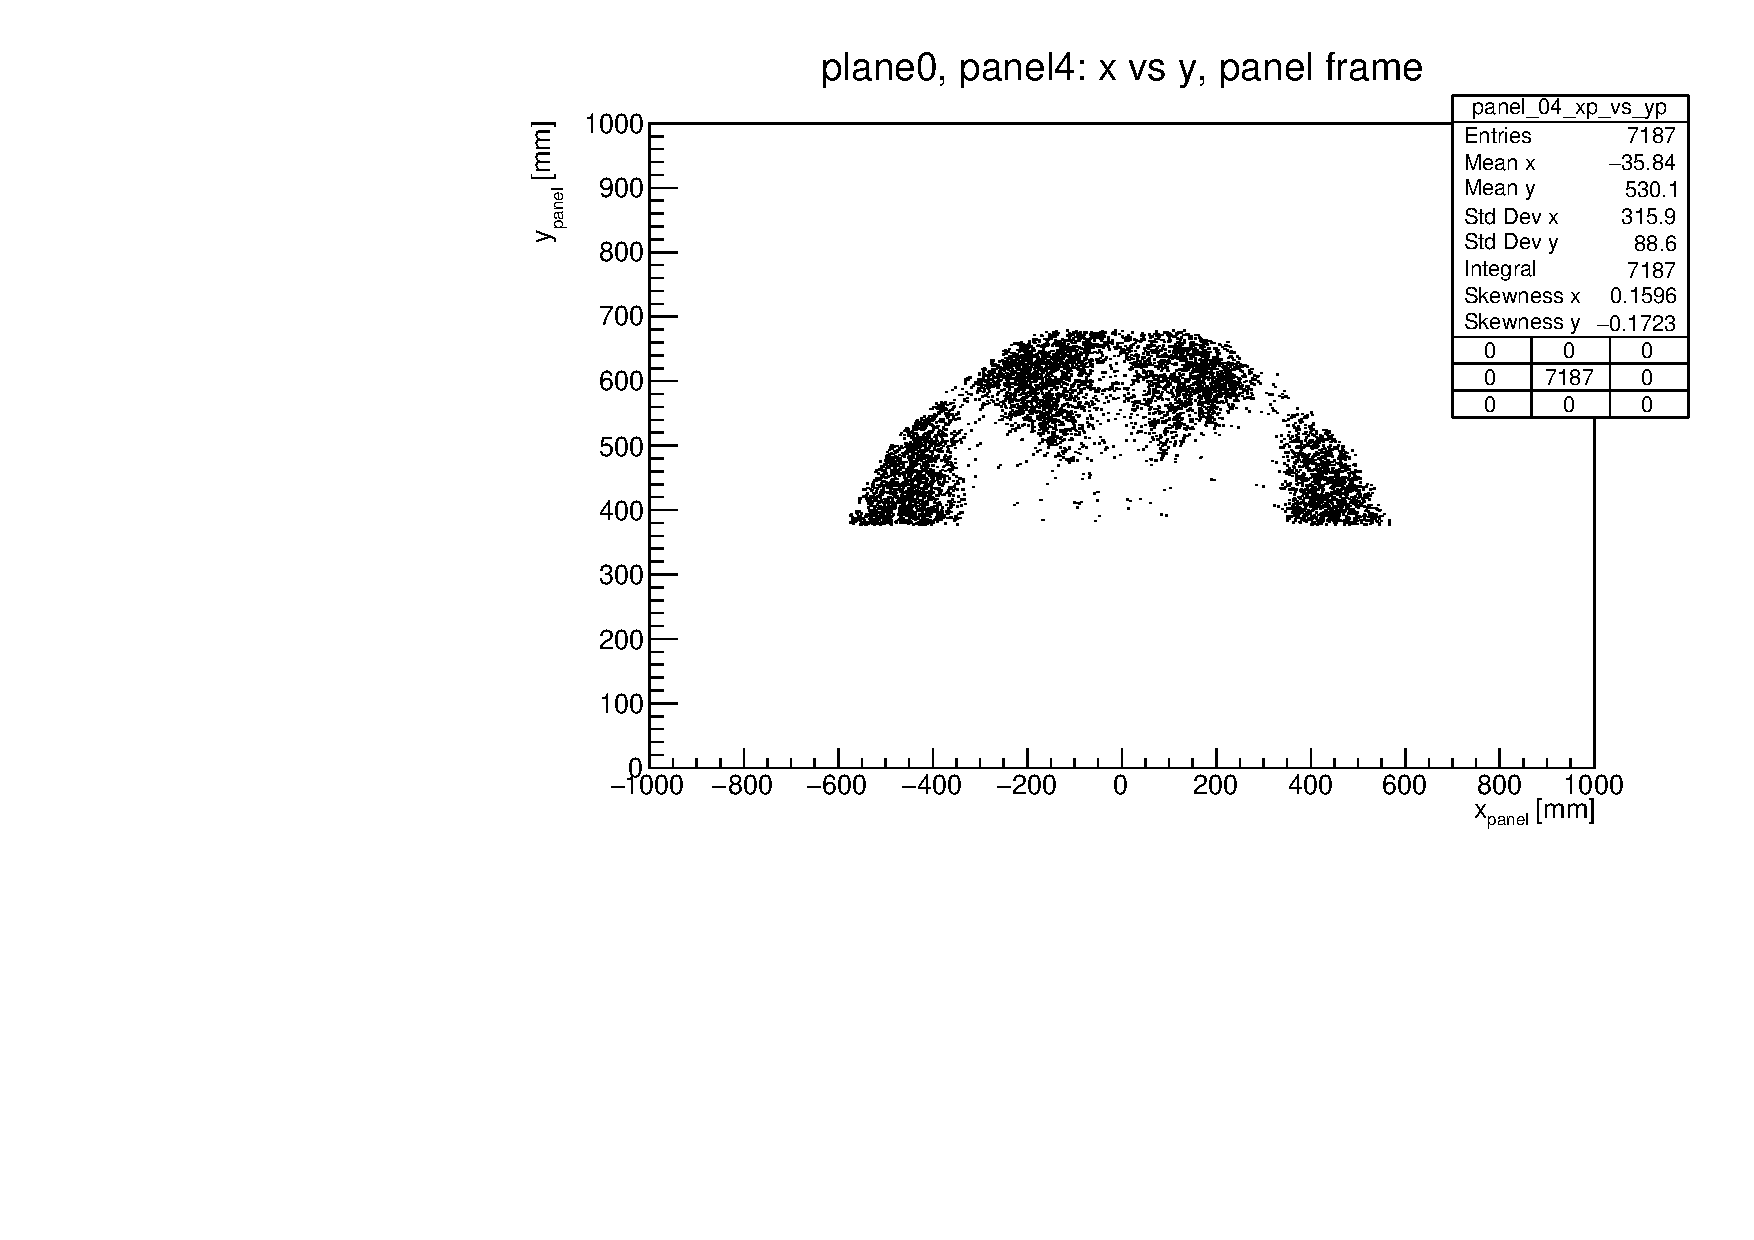
\includegraphics[width=0.95\textwidth]{figures/pdf/plane0_panel4_x_vs_y_all.pdf}
        %\caption{panel4}
        \label{fig:panel4plane0}
    \end{subfigure}
    \hfill
    \begin{subfigure}[b]{0.4\textwidth}
        \centering
        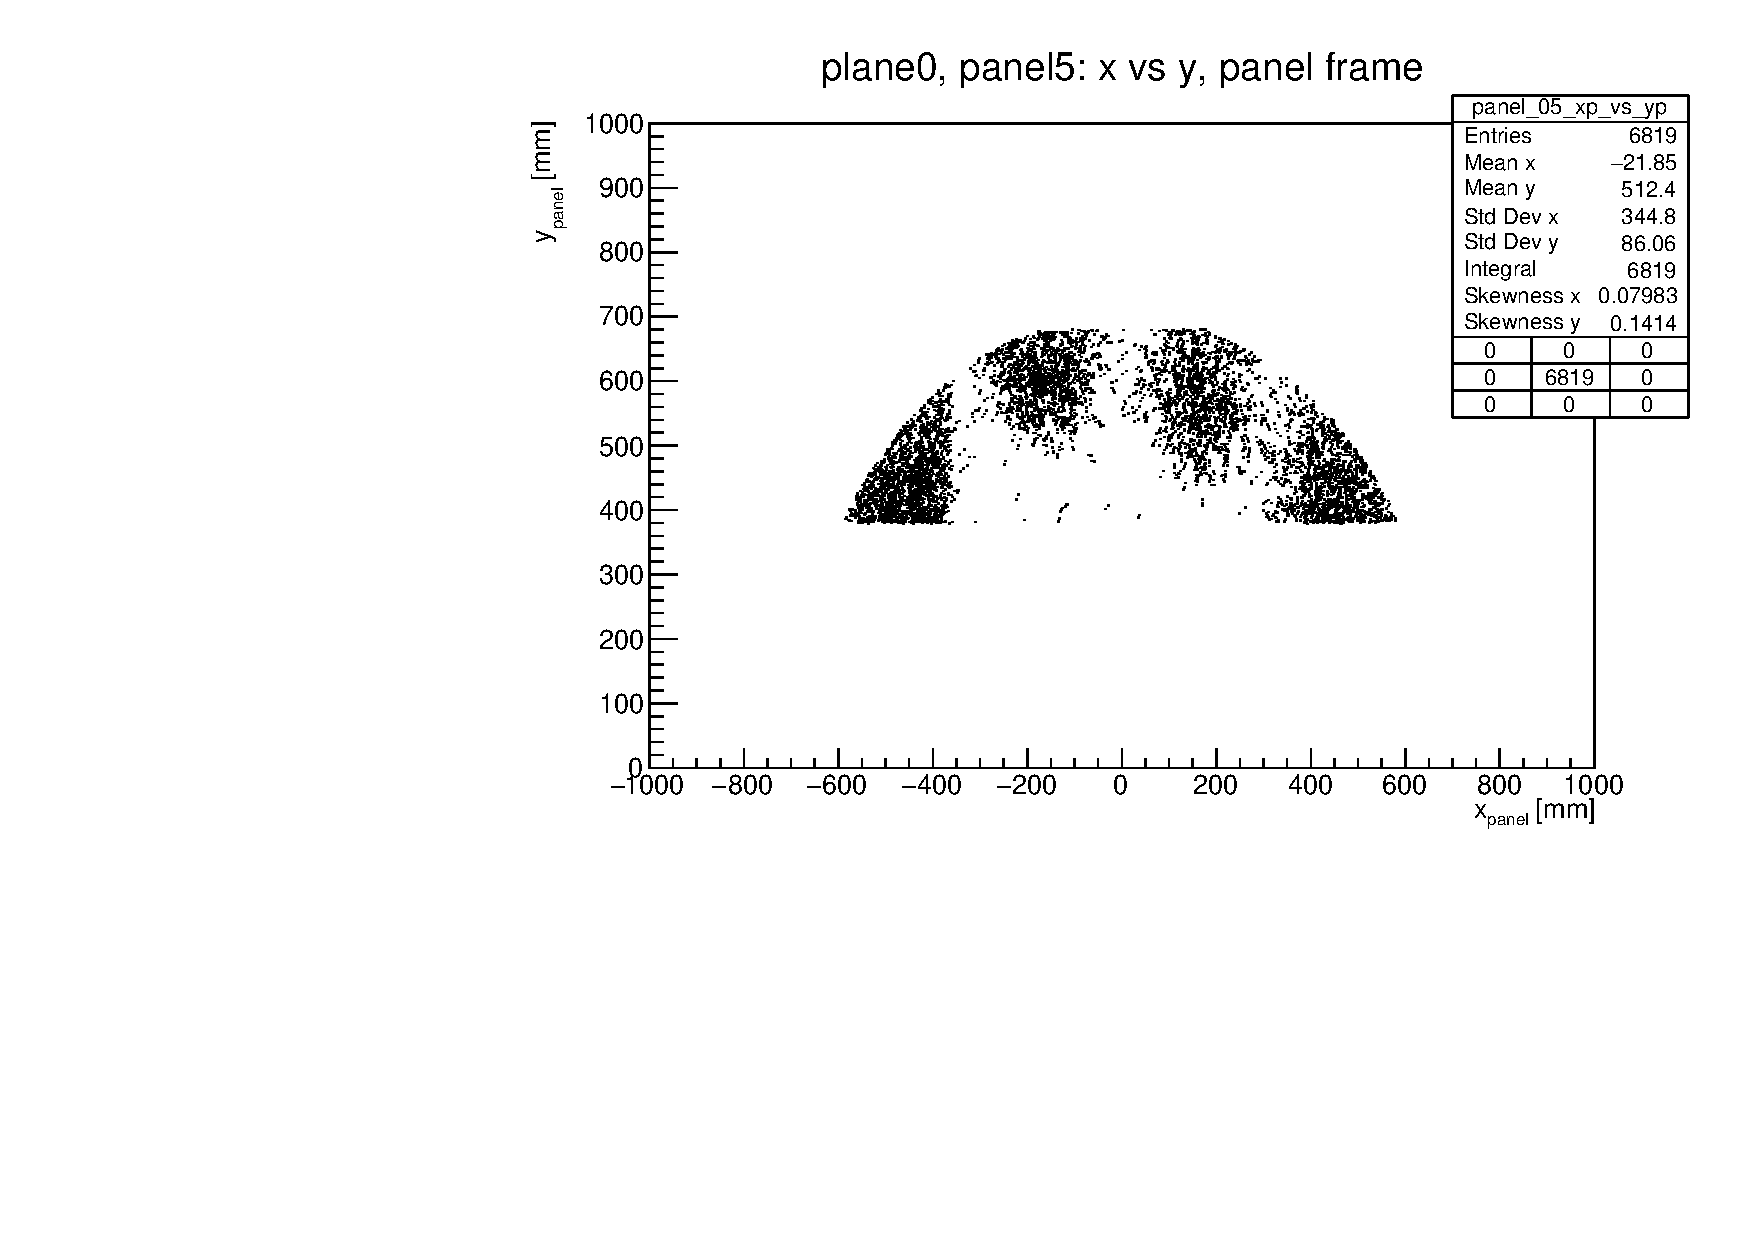
\includegraphics[width=0.95\textwidth]{figures/pdf/plane0_panel5_x_vs_y_all.pdf}
        %\caption{panel5}
        \label{fig:panel5plane0}
    \end{subfigure}
       \caption{Illumination pattern of cosmics hits on the panels of plane 0.}
       \label{fig:plane0}
\end{figure}
\begin{figure}[!h]
    \centering
    \begin{subfigure}[b]{0.4\textwidth}
        \centering
        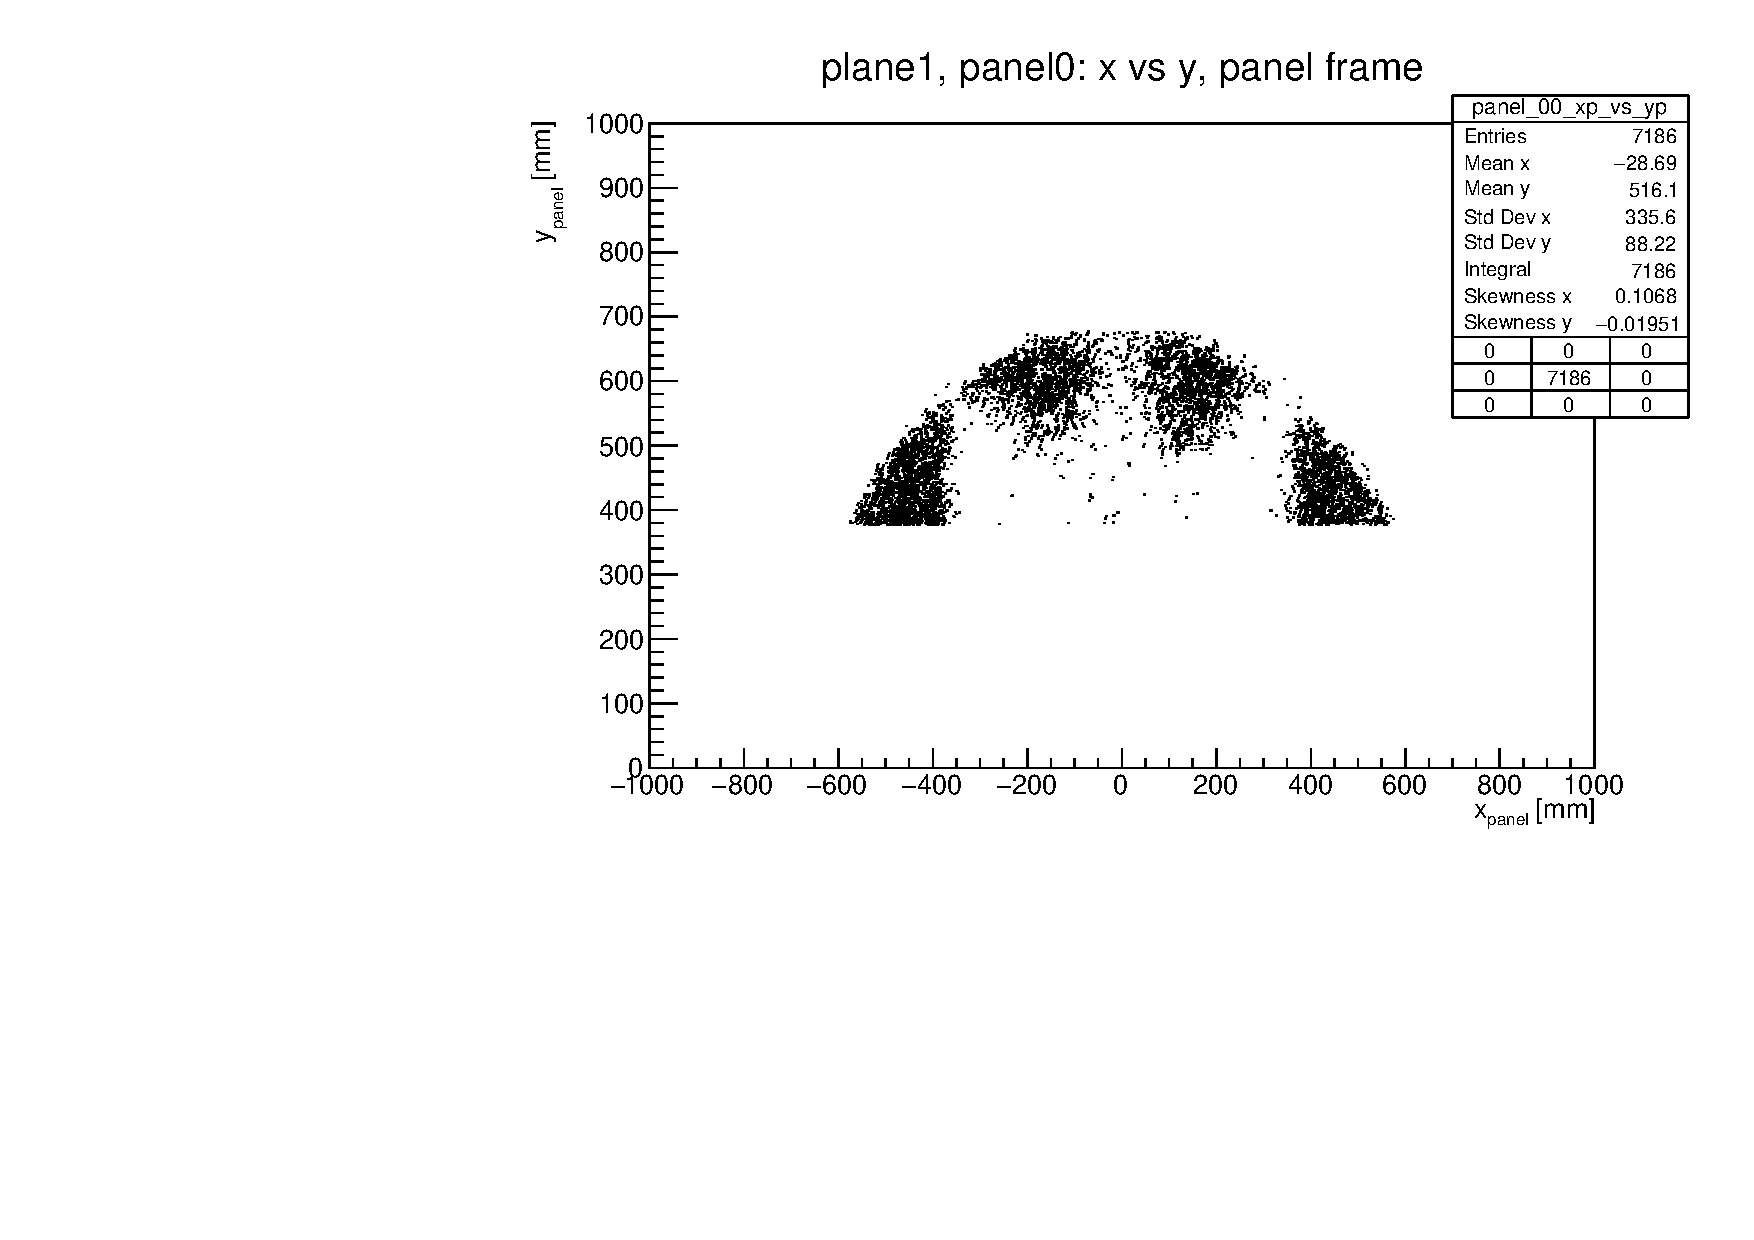
\includegraphics[width=0.95\textwidth]{figures/pdf/plane1_panel0_x_vs_y_all.pdf}
        %\caption{panel0}
        \label{fig:panel0plane1}
    \end{subfigure}
    \hfill
    \begin{subfigure}[b]{0.4\textwidth}
        \centering
        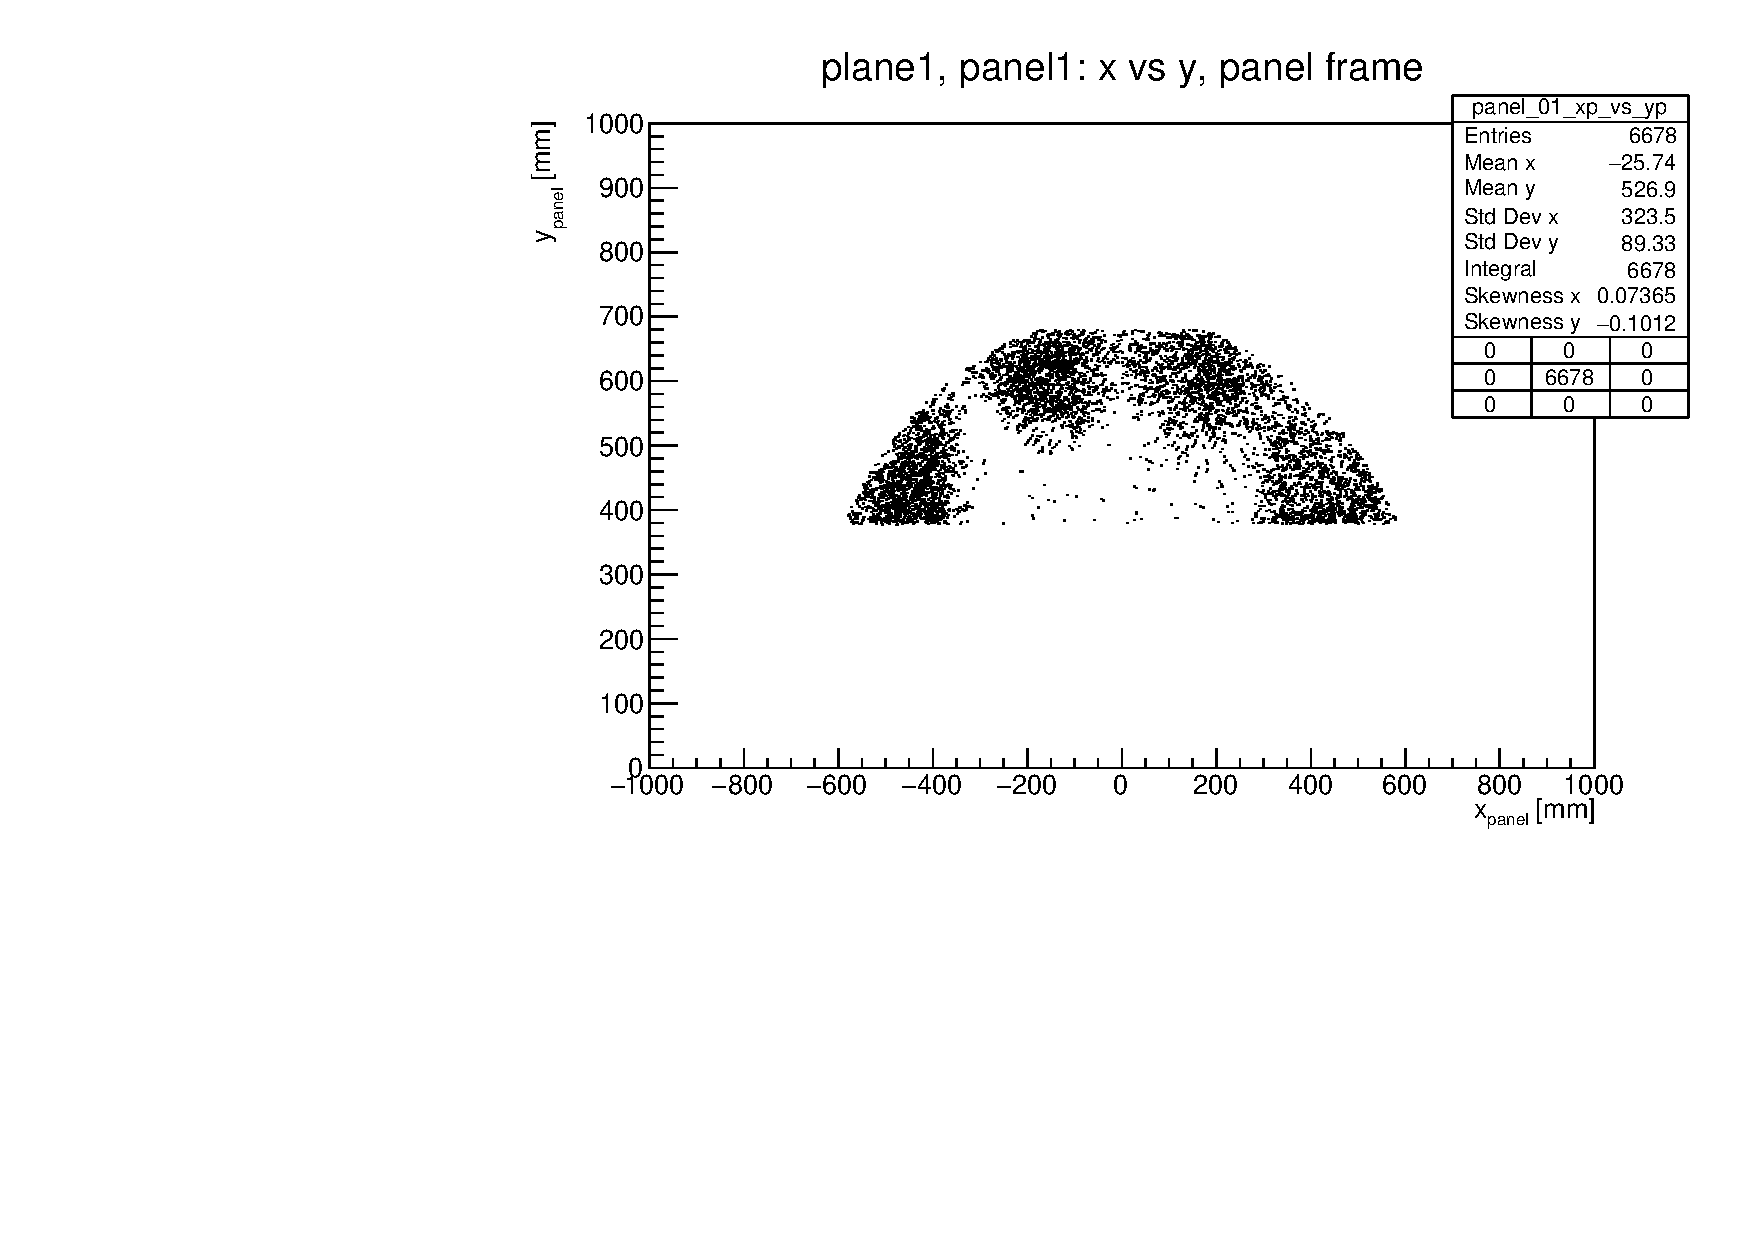
\includegraphics[width=0.95\textwidth]{figures/pdf/plane1_panel1_x_vs_y_all.pdf}
        %\caption{panel1}
        \label{fig:panel1plane1}
    \end{subfigure}
    \hfill
    \begin{subfigure}[b]{0.4\textwidth}
        \centering
        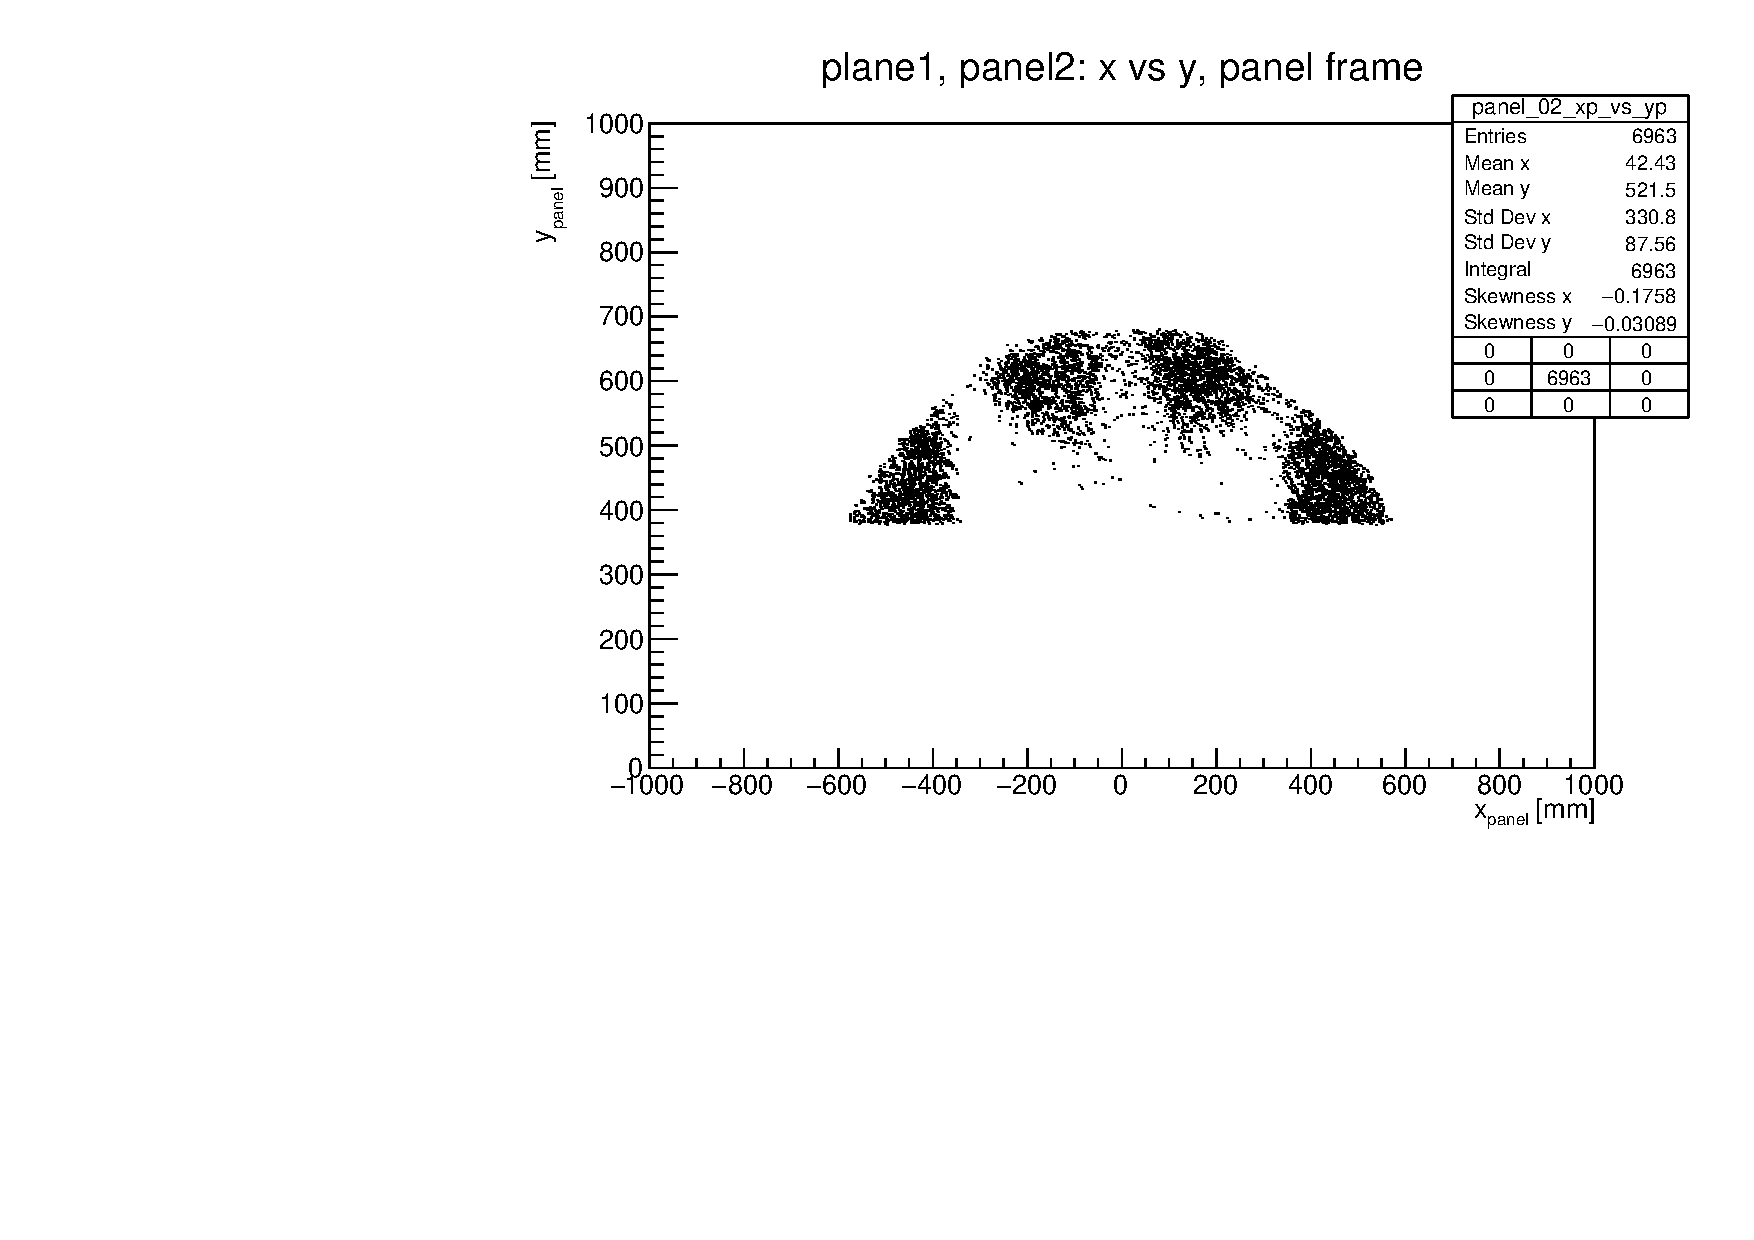
\includegraphics[width=0.95\textwidth]{figures/pdf/plane1_panel2_x_vs_y_all.pdf}
        %\caption{panel2}
        \label{fig:panel2plane1}
    \end{subfigure}
    \hfill
    \begin{subfigure}[b]{0.4\textwidth}
        \centering
        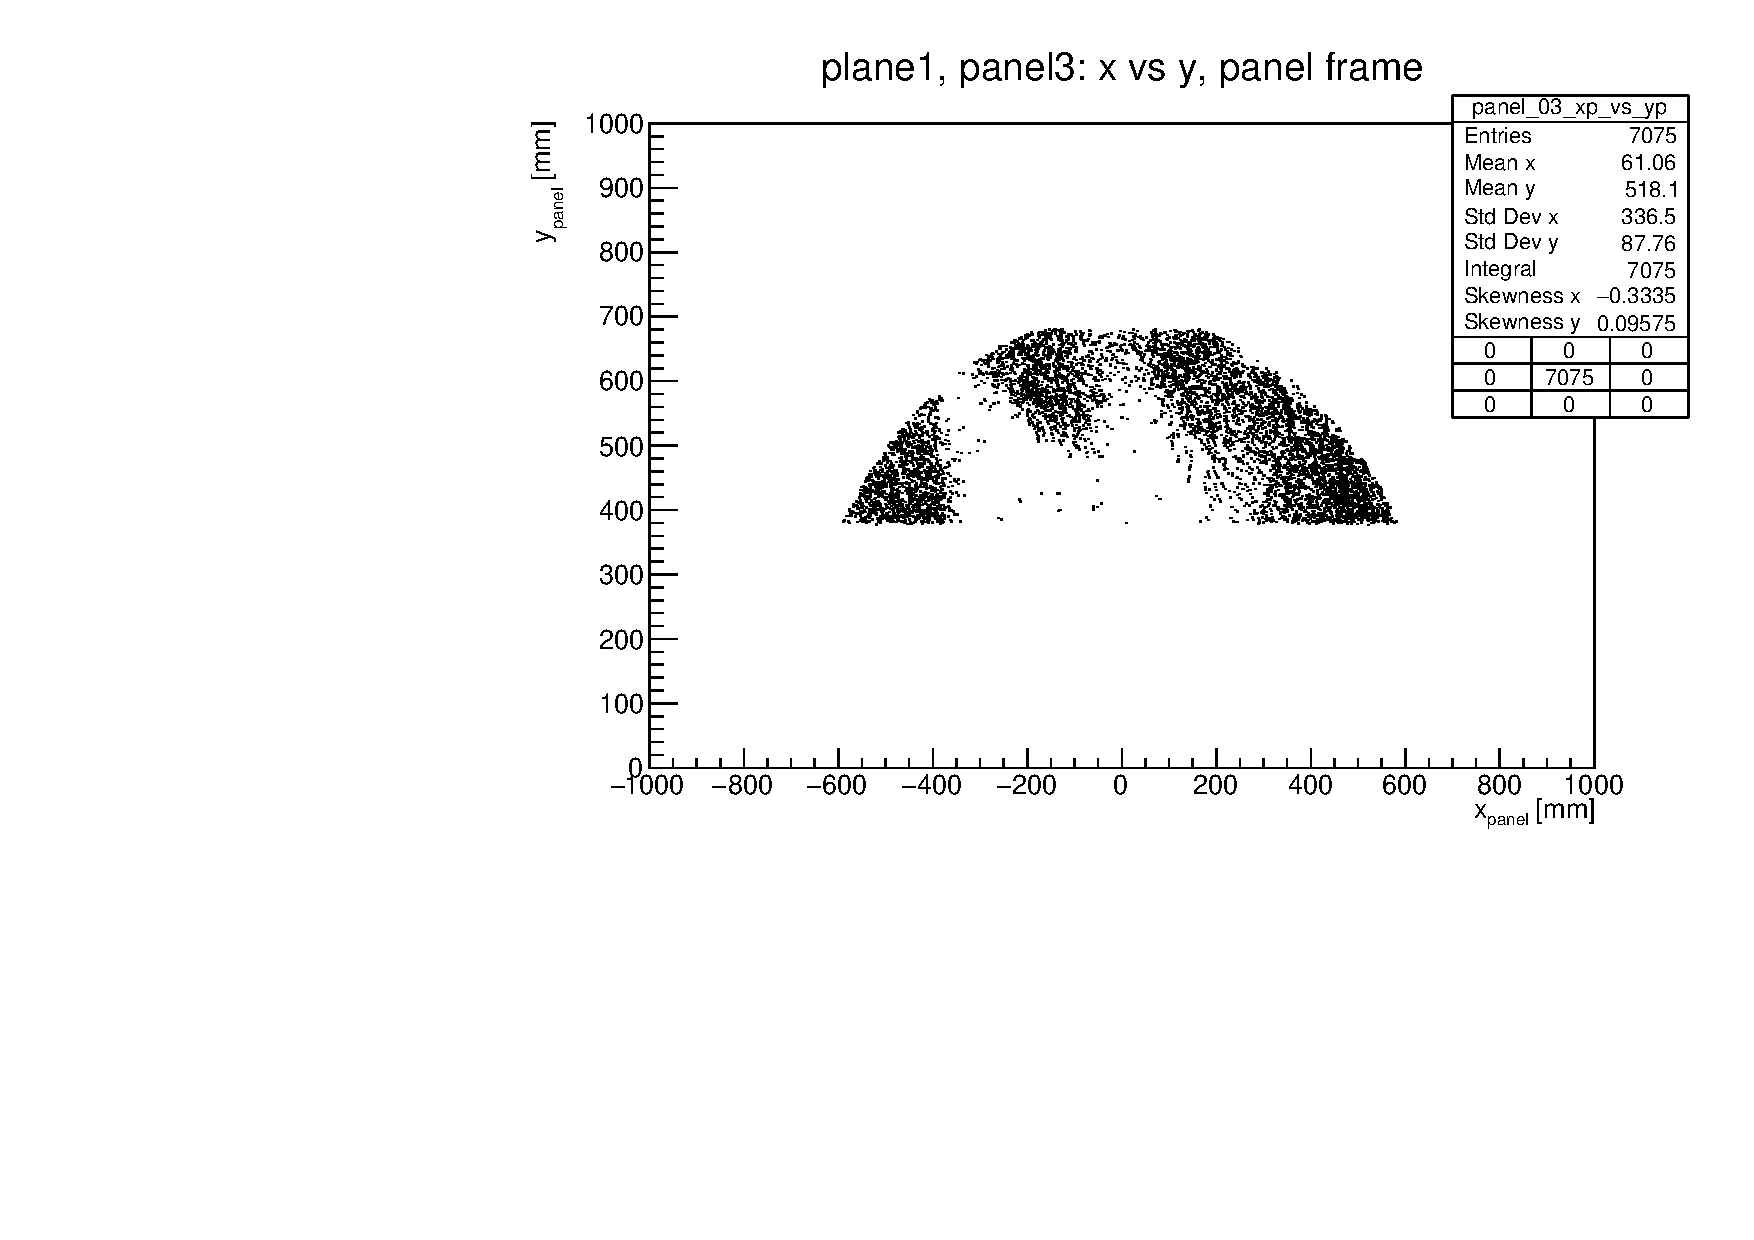
\includegraphics[width=0.95\textwidth]{figures/pdf/plane1_panel3_x_vs_y_all.pdf}
        %\caption{panel3}
        \label{fig:panel3plane1}
    \end{subfigure}
    \hfill
    \begin{subfigure}[b]{0.4\textwidth}
        \centering
        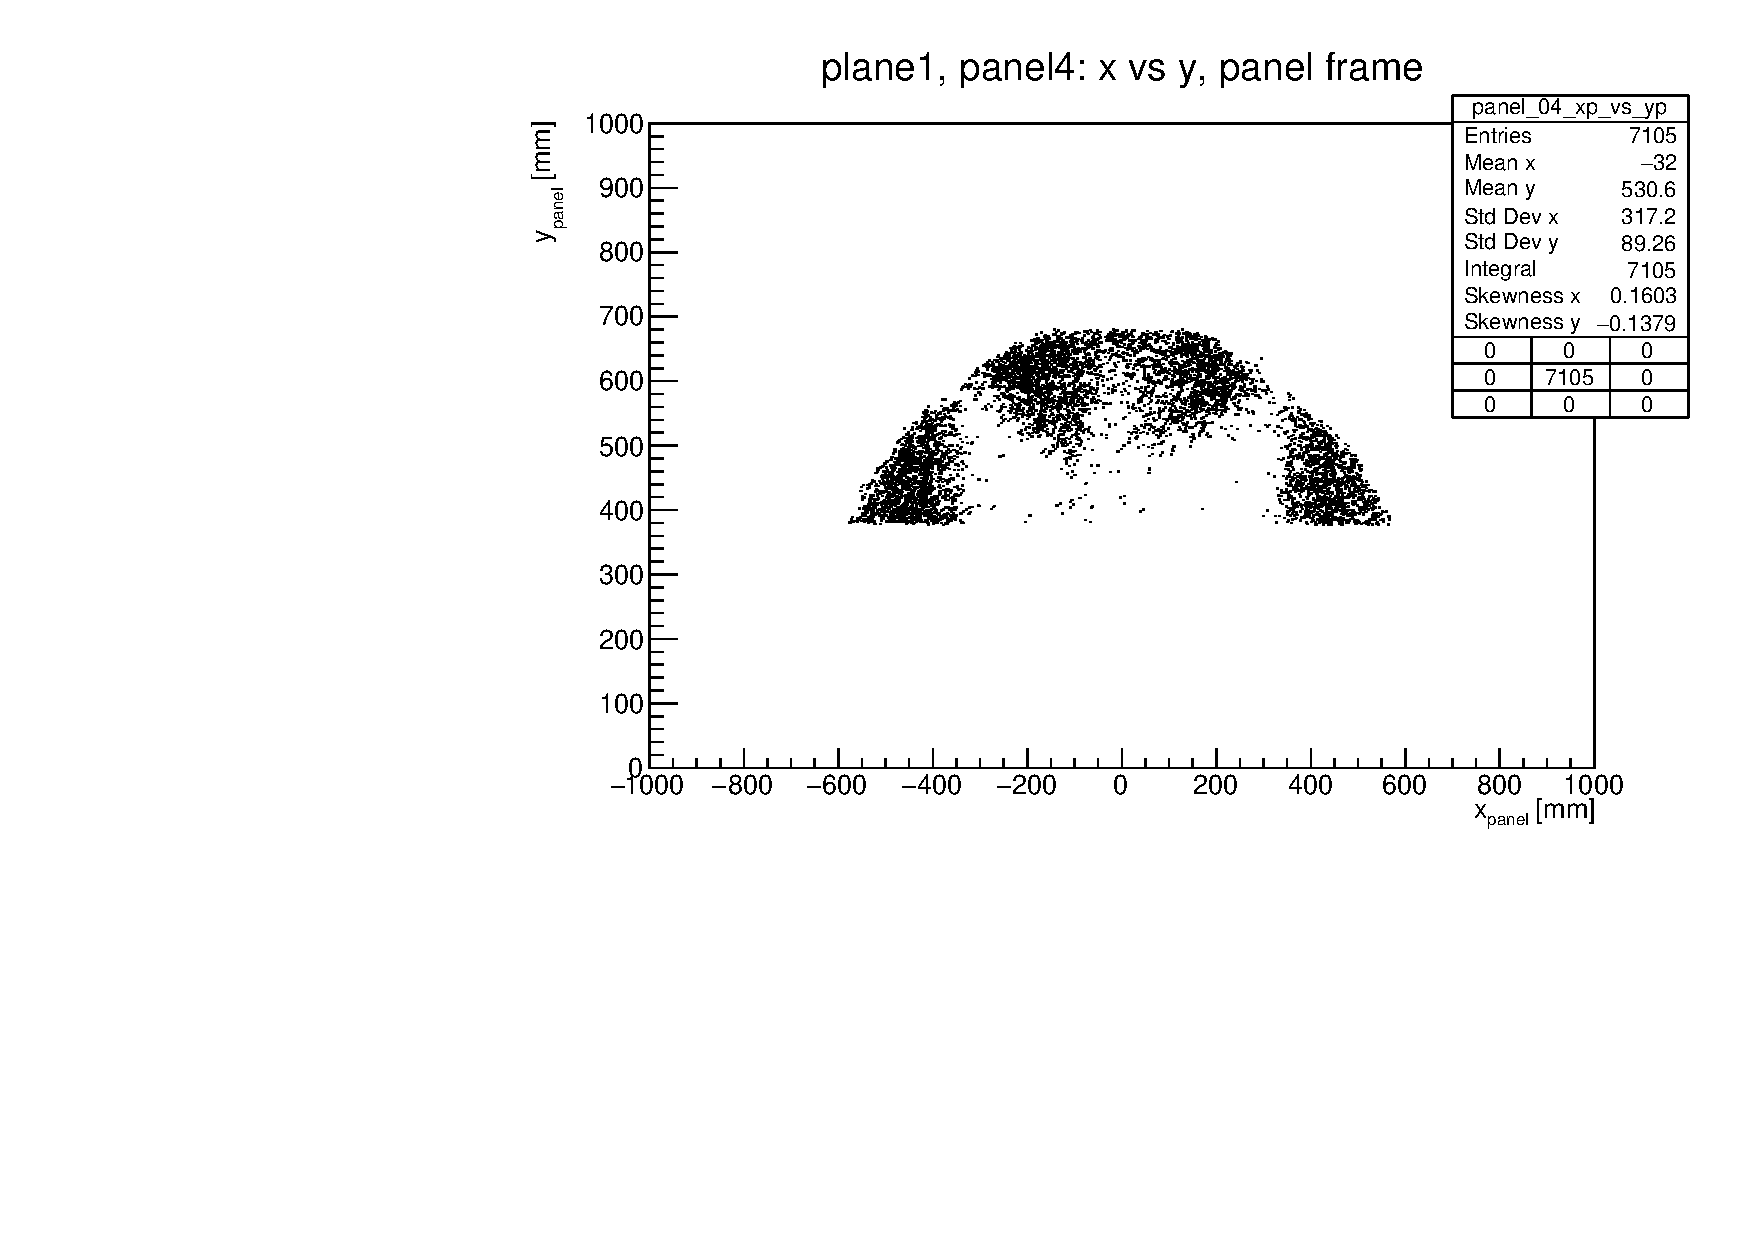
\includegraphics[width=0.95\textwidth]{figures/pdf/plane1_panel4_x_vs_y_all.pdf}
        %\caption{panel4}
        \label{fig:panel4plane1}
    \end{subfigure}
    \hfill
    \begin{subfigure}[b]{0.4\textwidth}
        \centering
        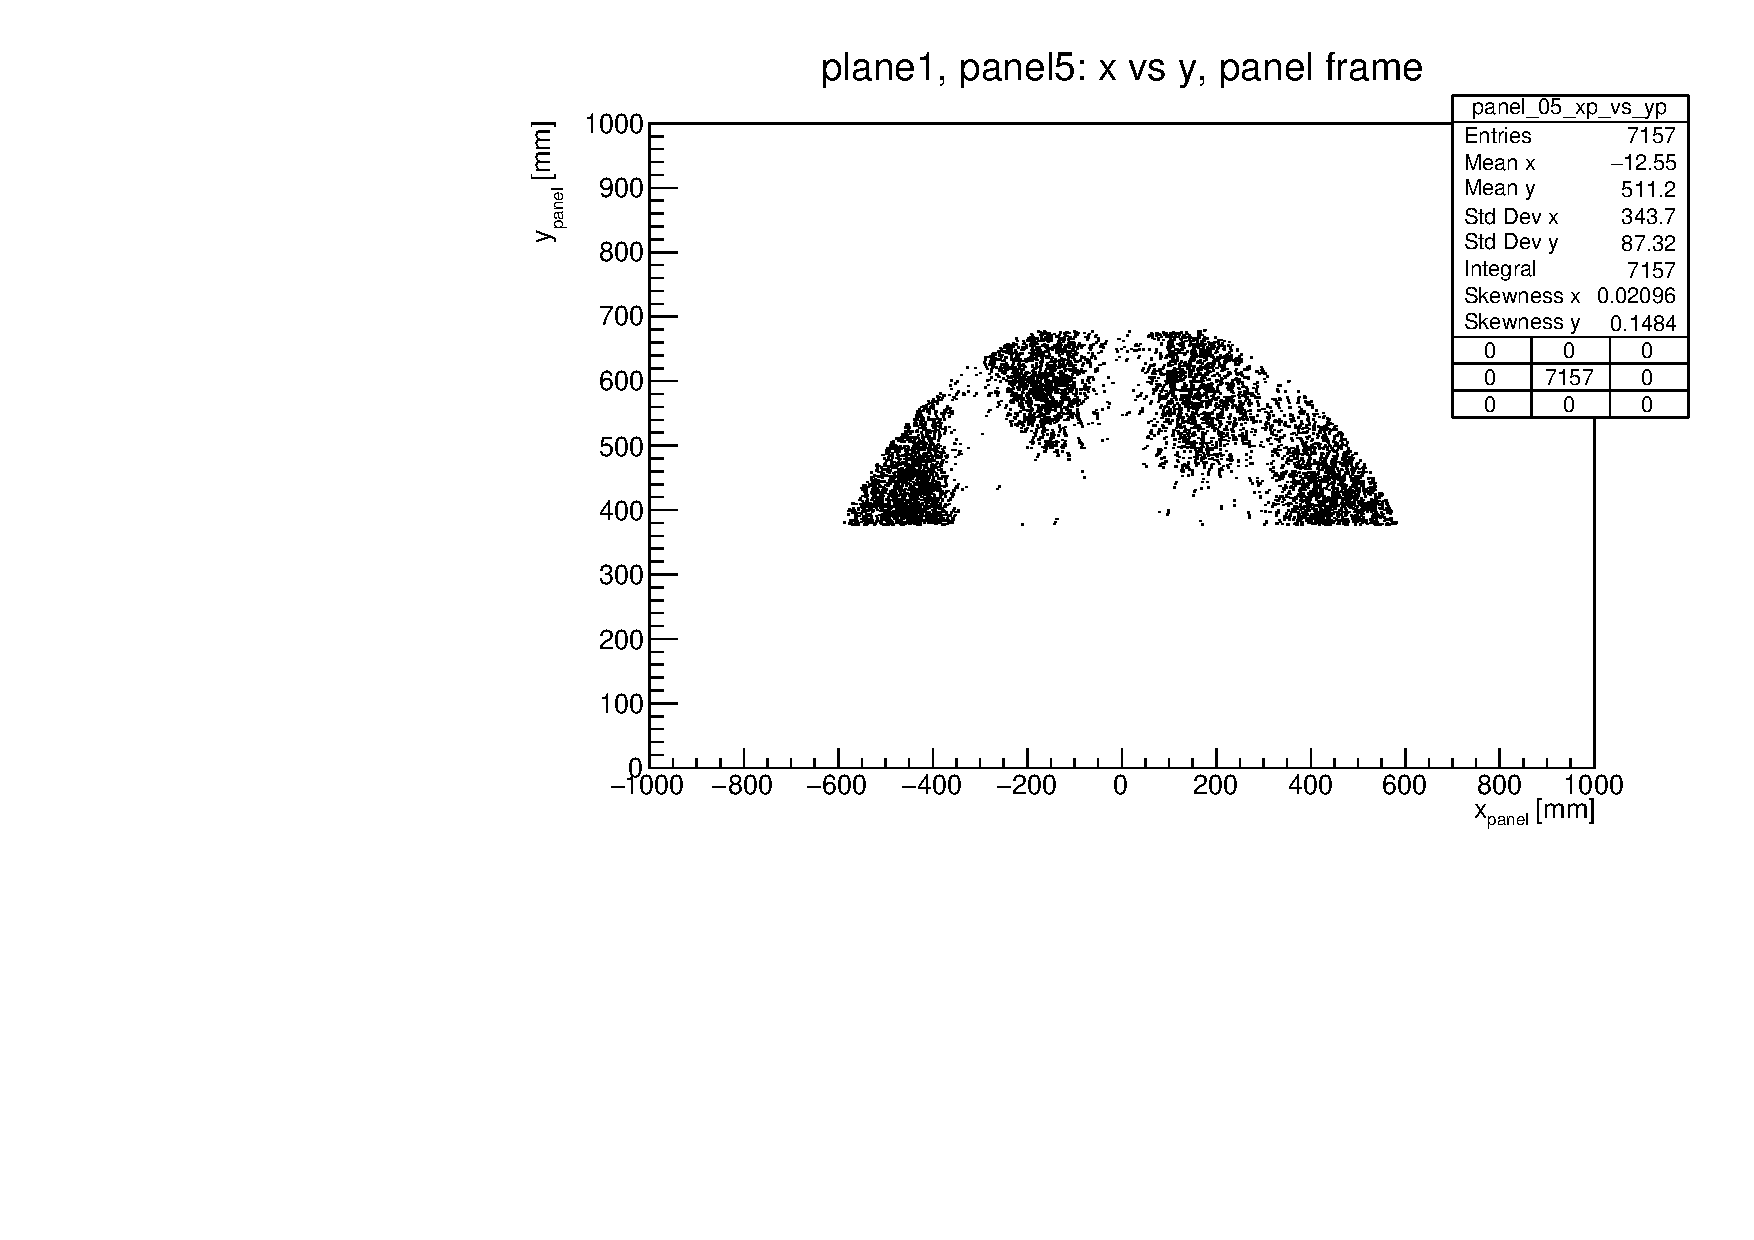
\includegraphics[width=0.95\textwidth]{figures/pdf/plane1_panel5_x_vs_y_all.pdf}
        %\caption{panel5}
        \label{fig:panel5plane1}
    \end{subfigure}
       \caption{Illumination pattern of cosmics hits on the panels of plane 1.}
       \label{fig:plane1}
\end{figure}